Use the sweat data in Table 5.1 (See Example 5.2.) Find simultaneous 95\% $T^{2}$ confidence
intervals for $\mu_{1}$, $\mu_{2}$, and $\mu_{3}$ using Result 5.3. Construct the 95\% Bonferroni intervals
using (5--29). Compare the two sets of intervals.
\newline
\newline
Copy the info from Exercise 5.4, $n=20$ observations, we find that
    \[
        \bar{\textbf{x}}
        =
        \begin{bNiceArray}{c}
            4.64 \\
            45.4 \\
            9.965
        \end{bNiceArray},
        \hspace{0.4cm}
        \textbf{S}
        =
        \begin{bNiceArray}{rrr}
            2.8794  &  10.01   & -1.8091 \\
            10.01   & 199.7884 & -5.64   \\
            -1.8091 &  -5.64   &  3.6277
        \end{bNiceArray}
    \]
    \[
        \textbf{S}^{-1}
        =
        \begin{bNiceArray}{rrr}
            0.5862  & -0.0221 & 0.2580 \\
            -0.0221 &  0.0061 & -0.0016 \\
            0.2580  & -0.0016 & 0.4018
        \end{bNiceArray}
    \]
Simultaneous 95\% $T^{2}$ confidence intervals:
    \[
        \bar{\textbf{x}}
        +
        \sqrt{
            \frac{(n-1)p}{(n-p)}
            F_{p, n-p}(\alpha)
        }
        \sqrt{
            \frac{1}{n}
            \text{Diag}(\textbf{S})
        }
        \otimes
        \begin{bNiceArray}{rr}
            -1 & 1
        \end{bNiceArray}
    \]
    \[
        \Rightarrow
        \begin{bNiceArray}{c}
            4.64 \\
            45.4 \\
            9.965
        \end{bNiceArray}
        +
        \sqrt{
            \frac{(20-1)3}{(20-3)20}
            F_{3, 20-3}(0.05)
        }
        \sqrt{
            \frac{1}{20}
            \begin{bNiceArray}{c}
                2.8794 \\
                199.7884 \\
                3.6277
            \end{bNiceArray}
        }
        \otimes
        \begin{bNiceArray}{rr}
            -1 & 1
        \end{bNiceArray}
    \]
    \[
        \Rightarrow
        \begin{bNiceArray}{c}
            4.64 \\
            45.4 \\
            9.965
        \end{bNiceArray}
        +
        3.2739
        \begin{bNiceArray}{c}
            0.37943171 \\
            3.16060454 \\
            0.42589071
        \end{bNiceArray}
        \otimes
        \begin{bNiceArray}{rr}
            -1 & 1
        \end{bNiceArray}
    \]
    \[
        \Rightarrow
        \begin{bNiceArray}{c}
            4.64 \\
            45.4 \\
            9.965
        \end{bNiceArray}
        +
        3.2739
        \begin{bNiceArray}{cc}
            -0.37943171 & 0.37943171 \\
            -3.16060454 & 3.16060454 \\
            -0.42589071 & 0.42589071
        \end{bNiceArray}
    \]
    \[
        \Rightarrow
        \begin{bNiceArray}{cc}
            3.3978  & 5.8822 \\
            35.0524 & 55.7476 \\
            8.5707  &11.3593
        \end{bNiceArray}
    \]
Written nicely as:
\begin{align*}
    3.3978  &\leq \mu_{1} \leq  5.8822 \\
    35.0524 &\leq \mu_{2} \leq 55.7476 \\
    8.5707  &\leq \mu_{3} \leq 11.3593
\end{align*}
\newline
95\% Bonferroni confidence intervals

\[
    \bar{\textbf{x}}
    +
    t_{n-1}(\alpha/(2m))
    \sqrt{
        \frac{1}{n}
        \text{Diag}(\textbf{S})
    }
    \otimes
    \begin{bNiceArray}{rr}
        -1 & 1
    \end{bNiceArray}
\]
\[
    \Rightarrow
    \begin{bNiceArray}{c}
        4.64 \\
        45.4 \\
        9.965
    \end{bNiceArray}
    +
    t_{20-1}(0.05/6)
    \sqrt{
        \frac{1}{20}
        \begin{bNiceArray}{c}
            2.8794 \\
            199.7884 \\
            3.6277
        \end{bNiceArray}
    }
    \otimes
    \begin{bNiceArray}{rr}
        -1 & 1
    \end{bNiceArray}
\]
\[
    \Rightarrow
    \begin{bNiceArray}{c}
        4.64 \\
        45.4 \\
        9.965
    \end{bNiceArray}
    +
    2.6251
    \begin{bNiceArray}{c}
        0.37943171 \\
        3.16060454 \\
        0.42589071
    \end{bNiceArray}
    \otimes
    \begin{bNiceArray}{rr}
        -1 & 1
    \end{bNiceArray}
\]
\[
    \Rightarrow
    \begin{bNiceArray}{c}
        4.64 \\
        45.4 \\
        9.965
    \end{bNiceArray}
    +
    2.6251
    \begin{bNiceArray}{cc}
        -0.37943171 & 0.37943171 \\
        -3.16060454 & 3.16060454 \\
        -0.42589071 & 0.42589071
    \end{bNiceArray}
\]
\[
    \Rightarrow
    \begin{bNiceArray}{cc}
        3.6440  & 5.6360 \\
        37.1031 & 53.6969 \\
        8.8470  & 11.0830
    \end{bNiceArray}
\]
Written nicely as:
\begin{align*}
    3.6440  &\leq \mu_{1} \leq 5.6360 \\
    37.1031 &\leq \mu_{2} \leq 53.6969 \\
    8.8470  &\leq \mu_{3} \leq 11.0830
\end{align*}

As expected, the Bonferroni intervals are slightly more narrow than the simultaneous $T^{2}$ intervals.
Here's a visual representation of that with the 2D simultaneous $T^{2}$ ellipses and the projections onto the component axes. The dotted lines are the simultaneous $T^{2}$ intervals and the dashed lines are the Bonferroni intervals.

\begin{figure}[H]
    \centering
    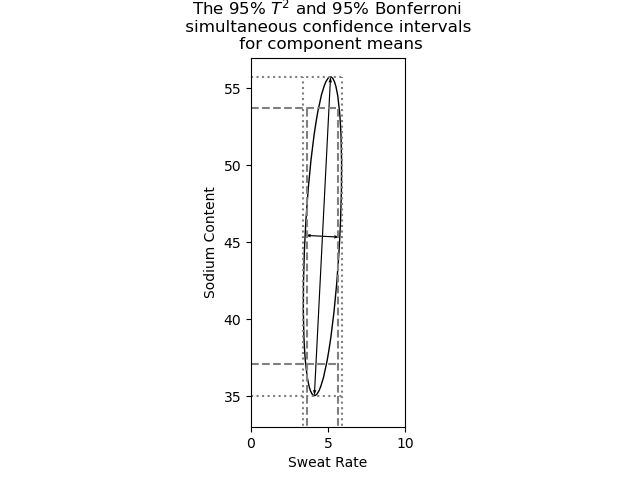
\includegraphics[scale=0.75]{./python/chapter-5/Question-5-7-CI-Sweat-Sodium.png}
\end{figure}

\begin{figure}[H]
    \centering
    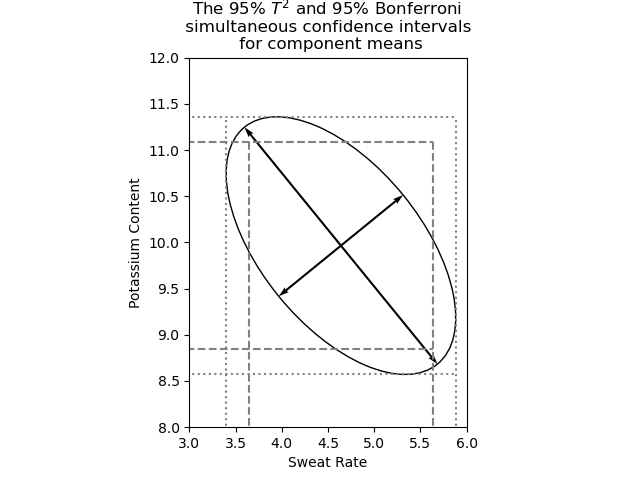
\includegraphics[scale=0.75]{./python/chapter-5/Question-5-7-CI-Sweat-Potassium.png}
\end{figure}

\begin{figure}[H]
    \centering
    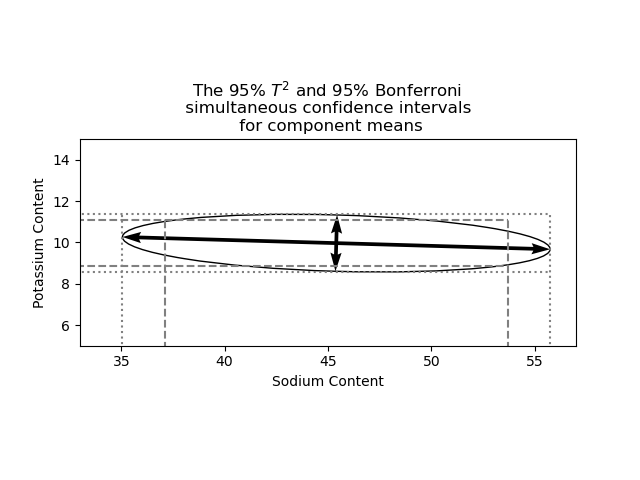
\includegraphics[scale=0.75]{./python/chapter-5/Question-5-7-CI-Sodium-Potassium.png}
\end{figure}

